% story.tex --- story-format companion draft of Paper B.
%
% This is a SEPARATE document from main.tex (draft of August 22, 2026), which is
% untouched and remains the technical report of record: it carries the appendix
% datasheet, the twin tables with every interval, the analysis-subset
% enumeration, and the complete prediction ledger. This version reorganises the
% SAME evidence around one alternative explanation and three predictions derived
% from it, in the manner of "Are Emergent Abilities of Large Language Models a
% Mirage?" (arXiv:2304.15004).
%
% Every number here is copied from main.tex / sections/ or the papers/analysis
% artifacts they cite. No number, claim, caveat, or registration status has been
% changed. Where a registered prediction failed, the failure is stated where the
% claim appears.

\documentclass[11pt]{article}
\usepackage[margin=1in]{geometry}
\usepackage{amsmath,amssymb}
\usepackage{graphicx}
\usepackage{booktabs}
\usepackage{array}
\newcolumntype{L}[1]{>{\raggedright\arraybackslash}p{#1}}
\usepackage{xcolor}
\usepackage[colorlinks=true,linkcolor=blue,citecolor=blue,urlcolor=blue]{hyperref}
\usepackage{caption}
\captionsetup{font=small,labelfont=bf}

\usepackage{placeins}
\renewcommand{\topfraction}{0.9}
\renewcommand{\bottomfraction}{0.8}
\renewcommand{\textfraction}{0.07}
\renewcommand{\floatpagefraction}{0.75}
\setcounter{topnumber}{3}
\setcounter{totalnumber}{5}

\newcommand{\tfa}{\textsc{TFA}}

\title{Matching Measures the Reference, Not the Solution}
\author{Anonymous Authors}
\date{Companion draft, September 1, 2026}

\begin{document}
\maketitle

\begin{abstract}
\noindent
Benchmarks ship a worked reference solution, and the cheapest way to grade a model's solution is to score how closely it matches that reference.
We propose one alternative reading of what such a score measures: it is dominated by a property of the \emph{reference}, how predictable its text is, rather than by any property of the solution in front of it, so it grades the answer key and not the student.
Three predictions follow, and we test each against blind human grades of reasoning soundness and against executed tests, across seventeen models from four families on eight math and code benchmarks plus an agentic setting.
First, no matching metric should be able to grade an individual solution, and none can: every metric we tested, from teacher-forced accuracy through sentence embeddings to a modern retrieval embedder and an NLI entailment model, lands in the band $[-0.33, +0.14]$ against human soundness, and the sole signal escaping the band compares extracted final answers, which is the free correctness bit under another name.
Second, the dominant share of a matching score's per-solution variance should belong to the reference, and it does, $83$--$92\%$ for the prediction-fit metrics, an item effect that replicates across model families and survives item resampling and single-model deletion.
Third, matching should rank models exactly where the reference is worth predicting, and the boundary lands as predicted: rankings run strongly positive on olympiad benchmarks, invert in sign on saturated grade-school data, and collapse on the same items when the worked reference is replaced by its bare answer line or by length-matched boilerplate.
What does carry signal never treats the reference as a similarity target, and nothing cheap beats the check everyone already has: the machine-checked answer-correct bit alone correlates $+0.92$ with human soundness, and our strongest verification signal, a completion-based curve, sits significantly below it on paired items and adds no measurable grading signal beyond it.
Three rules follow: check the final answer before buying any deeper signal, use a reference only as a checkable endpoint and never as a similarity target, and report reference perplexity alongside accuracy, because matching is legitimate exactly when references are worth predicting.
\end{abstract}

\begin{table}[t!]
\centering
\small
\setlength{\tabcolsep}{5pt}
\begin{tabular}{L{1.1cm}L{4.6cm}L{4.2cm}L{4.0cm}}
\toprule
& Prediction & Test & Result \\
\midrule
\textbf{P1} & No matching metric can grade an individual solution, structurally so for metrics that never read it &
Five metrics plus four stronger baselines against blind human soundness on a fixed anchor set, and against executed tests on code &
\textbf{Everything lands in $[-0.33, +0.14]$}; the sole escape reads only final answers, the free correctness bit in disguise (Section~\ref{sec:p1}) \\
\addlinespace[3pt]
\textbf{P2} & The dominant share of a matching score's per-solution variance is a property of the reference, not the solution &
Cross-family fixed-effects decomposition on four benchmarks with resampling and deletion checks; two reference interventions; two registered repairs &
\textbf{$83$--$92\%$ (prediction fit)} and $45$--$70\%$ (similarity) is reference-side and stable; swapping the reference for an answer line or padded boilerplate collapses the signal (Section~\ref{sec:p2}) \\
\addlinespace[3pt]
\textbf{P3} & Matching can rank models, but only in aggregate and only where the reference is worth predicting &
A nine-benchmark boundary map, twelve hard-side and twelve saturated family ladders, and an agentic setting &
\textbf{$\rho$ runs $+0.86$ to $-0.25$} from olympiad to saturated; 12 of 12 hard ladders positive, 5 of 12 saturated ladders invert (Section~\ref{sec:p3}) \\
\midrule
\emph{Signal} & Signals that verify a checkable endpoint carry signal, and none beats the endpoint itself &
The free answer-correct bit, a thirty-two-rollout completion curve, and an answer-swap margin on the same anchors &
\textbf{The free bit reads $+0.92$}; the curve loses to it on paired items and adds nothing given the bit (Section~\ref{sec:verify}) \\
\bottomrule
\end{tabular}
\caption{\textbf{Takeaway: one explanation, three predictions, three confirmations, and a constructive remainder that is already free.} The explanation is that a matching score is dominated by how predictable the reference text is, so it measures the answer key rather than the student. Correlations are against blind human soundness on the anchor set unless a ranking is named; intervals, subset sizes, and per-row caveats are in the tables of the sections named. Six directional predictions were registered in advance and four landed as called; the two misses, a sign flip and a falsification, are reported inline where they bite (Sections~\ref{sec:repairs} and~\ref{sec:verify}).}
\label{tab:predictions}
\end{table}

\section{Introduction}
\label{sec:intro}

A benchmark ships a worked reference solution for every problem, and the cheapest grader scores a model's solution by its similarity to that reference.
A student who writes a beautiful wrong derivation matches the reference well; a student who solves the problem an unusual correct way matches it badly.
The intuition that keeps the practice alive is that similarity degrades gracefully, so a cheaper metric measures the same thing a judge measures, only with more noise.
Figure~\ref{fig:class} shows what we find instead: every matching metric we tested straddles zero against blind human grades of reasoning soundness, on solutions where the free answer-correct bit reads $+0.92$, and the gap between those two facts is this paper.

\begin{figure}[t!]
\centering
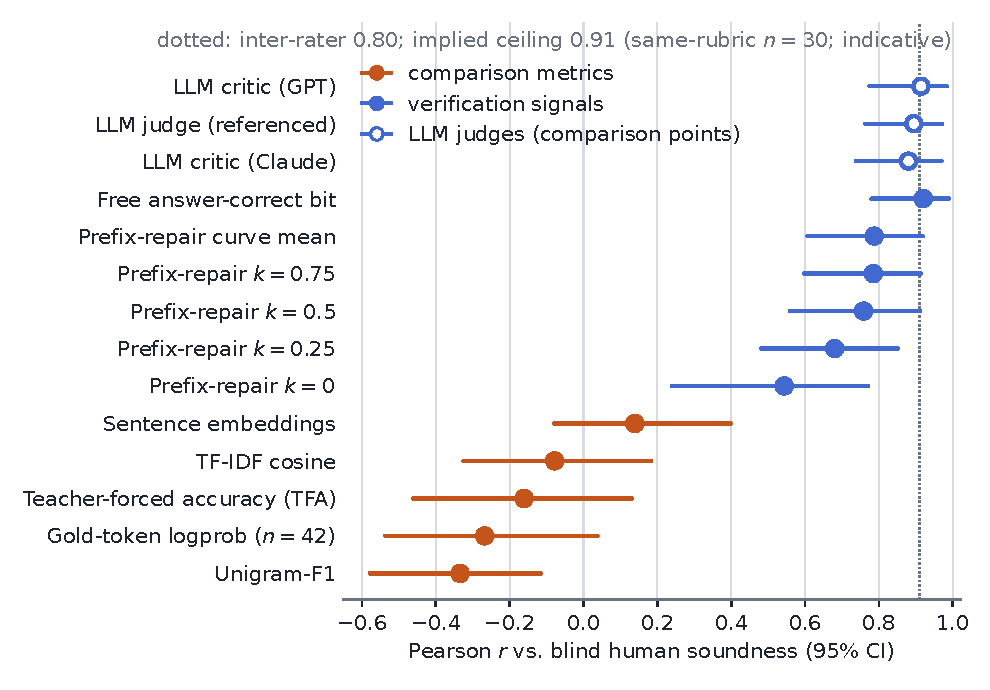
\includegraphics[width=0.84\textwidth]{figures/fig_class.pdf}
\caption{\textbf{Takeaway: every matching metric straddles zero or sits weakly negative against blind human soundness, while the verification signals carry real signal, and the top of the field is the bit everyone already has for free at $+0.92$.}
Pearson correlation with blind human soundness on the 60-item anchor set, with bootstrap 95\% CIs: matching metrics in orange, verification signals in blue, LLM judges (expensive comparison points) as hollow markers.
Unigram-F1's CI excludes zero on the negative side, uncorrected for the five-metric battery, so that single exclusion is suggestive rather than confirmatory.
Dotted lines mark the inter-rater agreement and the implied single-rater ceiling; both reliability estimates have wide intervals, so ceiling comparisons are indicative only.}
\label{fig:class}
\end{figure}

The appeal is real.
A matching score is deterministic, costs one forward pass, involves no judge prompt whose wording could shift the score, and anyone can audit it.
The sharpest such metric is teacher-forced accuracy (\tfa): feed the model the problem and the gold solution one token at a time, and score the fraction of gold tokens the model would have predicted itself.
\tfa{} was introduced as a judge-free evaluation signal by \textsc{Putnam-AXIOM}~\cite{gulati2025putnam}; we do not introduce it here, we characterize it, together with the rest of the matching family, from gold-token log-probability through TF-IDF, unigram-F1, and sentence embeddings, on benchmarks from grade-school math to program synthesis~\cite{cobbe2021gsm8k,hendrycks2021math,chen2021codex}.
Prior work organizes this space along a single axis of cost versus quality, string and embedding metrics at the cheap end~\cite{yuan2021bartscore} and LLM judges at the expensive end~\cite{zheng2023judging}, with the practical question being how far down the cost axis one can afford to go.

\paragraph{One alternative explanation.}
We propose that the cost--quality axis is the wrong axis, because a matching score is not a noisy grade at all.
It is dominated by a property of the \emph{reference}: how predictable this particular gold text is.
That quantity is fixed before any solution is generated, is identical for every model answering the same item, and has nothing to do with the solution being graded, so a score built on it measures the answer key rather than the student.
Everything in this paper follows from that single reading, and the operative distinction it induces is one of mechanism rather than cost: signals that score resemblance to the reference text (\emph{matching}) behave differently in kind from signals that check whether the solution reaches a checkable endpoint (\emph{verification}), at every price point we tried.

\paragraph{Three predictions.}
If the score belongs to the reference, three things must be true, and each fails under the noisy-grade reading.
\begin{itemize}
\item \textbf{P1.} No matching metric can grade an individual solution. A quantity owned by the reference cannot separate a sound solution from an unsound one on the same item; for the prediction-fit metrics, which never read the generated solution at all, the null is structural, a property of the metric's type signature, and for the output-similarity metrics it is an empirical claim the noisy-grade reading rejects (Section~\ref{sec:p1}).
\item \textbf{P2.} The dominant share of a matching score's per-solution variance must be an item effect, identical across model families, stable under resampling and model deletion, and interpretable as reference predictability; and removing or replacing the reference's information must destroy whatever signal remains, while no reweighting of reference tokens can recover a grade, because there is nothing solution-side to recover (Section~\ref{sec:p2}).
\item \textbf{P3.} Matching can still rank \emph{models}, but only in aggregate, where the per-item nuisance cancels, and only where the reference is worth predicting; on saturated benchmarks, where every model predicts the reference about equally well, the leftover is style and the ranking may invert in sign. The same metric must therefore dissociate cleanly: null at the item level and positive at the model level on the same benchmarks (Section~\ref{sec:p3}).
\end{itemize}

The explanation also states what \emph{does} grade, which separates it from blanket skepticism about cheap evaluation: any signal that uses the reference only as a checkable endpoint escapes the nuisance, and the cheapest such signal, comparing final answers, is free wherever references exist.
Section~\ref{sec:verify} tests the constructive half and finds its ordering surprising in one respect the registration did not call: the free bit tops the entire field, and even a thirty-two-rollout completion curve adds nothing beyond it.

\paragraph{Registration.}
Six directional predictions were registered before the data they are scored on existed: analysis scripts and predictions were committed to the repository before the corresponding runs, carrying first-party git timestamps.
Four of six landed as called, and we report the two misses where they bite rather than in a footnote: the position-weighting repair was registered as a null and produced a sign flip instead (Section~\ref{sec:repairs}), and the completer-strength register was falsified by a flat curve across a twenty-fold completer-size range (Section~\ref{sec:verify}).
The four stronger matching baselines of Section~\ref{sec:p1} were added post hoc in response to review and carry no registration weight, and we say so there.
The complete ledger, with per-leg verdicts, lives in Table~\ref{tab:ledger} and in the technical report version of this paper, together with every interval, subset enumeration, and instrument this document quotes.\footnote{Technical report version, draft of August 22, 2026, released with the code. It carries the appendix datasheet, the twin table with every confidence interval, the analysis-subset enumeration, the reliability cells, and the deferred-numbers table. This document reorganises the same evidence and changes no number.}
Table~\ref{tab:predictions} summarises the explanation, the three tests, and their outcomes.

\section{Setup}
\label{sec:setup}

\begin{table}[t!]
\centering
\footnotesize
\setlength{\tabcolsep}{2.5pt}
\begin{tabular}{llcc}
\toprule
benchmark & regime & cross-family $\rho$ [95\% CI] & within-family $\rho$ \\
\midrule
\textsc{Omni-MATH} & olympiad & $\mathbf{+0.86}$ $[+0.35, +1.00]$ & $+0.90$ \\
\textsc{Putnam-AXIOM} & olympiad & $+0.60$ $[+0.17, +0.83]$ & $\mathbf{+1.00}$ \\
\textsc{Putnam-Variations} & olympiad, contamination-proof & $+0.38$ $[-0.15, +0.73]$ & $+0.90$ \\
\textsc{HumanEval} & code & $+0.43$ $[-0.02, +0.76]$ & $+0.80$ \\
\textsc{MATH-500} & competition math & $+0.35$ $[-0.15, +0.71]$ & $+0.90$ \\
\textsc{MATH} (full) & competition math, near-saturated & $+0.21$ $[-0.29, +0.61]$ & $+0.60$ \\
\textsc{GSM8K} & grade school, saturated & $-0.25$ $[-0.71, +0.33]$ & $+0.70$ \\
\textsc{GSM8K-Platinum} & grade school, relabeled & $-0.19$ $[-0.71, +0.41]$ & $+0.60$ \\
\textsc{SWE-bench Verified} & agentic code, preliminary & $0.00$ (8 coder models) & $+1.00$ (Qwen-Coder, $n{=}4$) \\
\bottomrule
\end{tabular}
\caption{\textbf{Takeaway: the boundary map. Mean \tfa{} ranks models on hard benchmarks with information-dense references, degrades through code, and inverts in sign on saturated grade-school data, exactly where the reference stops being worth predicting.}
Cross-family Spearman correlation between mean \tfa{} and accuracy per benchmark (11--17 models by row; \textsc{Omni-MATH} uses a seven-model sweep and \textsc{SWE-bench} eight coder models; bootstrap 95\% CIs); the within-family column is the Qwen size ladder specifically.
Within-family Spearmans sit on ladders of three to five models, so the statistic takes only a few discrete values: read signs and consistency, not magnitudes.
The saturated-benchmark intervals are wide and straddle zero, so the sign inversion is a point-estimate trend; the robust statement is the ladder count of Section~\ref{sec:p3}, twelve of twelve hard-side ladders positive and five of twelve saturated ladders inverting.
The \textsc{SWE-bench} within-family entry is a four-model ladder and a preliminary observation.}
\label{tab:map}
\end{table}

\paragraph{Models and data.}
Seventeen instruction-tuned models from four families (Qwen, Phi, OLMo, and Mistral), spanning 0.5B to 32B parameters; math and edition variants (Qwen-Math, Ministral, Mathstral) count within their base families, and every cross-family claim uses these four families.
Eight benchmarks: \textsc{MATH-500} and full \textsc{MATH}~\cite{hendrycks2021math}, \textsc{Putnam-AXIOM} and its variations~\cite{gulati2025putnam}, \textsc{Omni-MATH}, \textsc{GSM8K}~\cite{cobbe2021gsm8k}, \textsc{GSM8K-Platinum}, and \textsc{HumanEval}~\cite{chen2021codex}/\textsc{MBPP+}~\cite{austin2021mbpp,liu2023evalplus}, plus \textsc{SWE-bench Verified} as an agentic setting, with patch-level \tfa{} over a separate grid of eight coder models.
Every model generates its own solution to every problem (greedy), and is separately teacher-forced on the gold solution.

\paragraph{Matching metrics.}
Five ways of scoring a solution against the reference, chosen to span the space: \tfa{} (hard argmax match on gold tokens), gold-token log-probability (the soft version of \tfa), TF-IDF cosine, unigram-F1, and sentence-embedding cosine.
The first two measure the model's predictive fit to the reference text and never read the generated solution; the last three measure how much the model's own output resembles it.
The recurring reference-side quantity is \emph{reference perplexity}: how hard the reference text is to predict, measured as bits-per-character under the scoring model.

\paragraph{Verification signals.}
Three judge-free signals consume the reference only through a checkable endpoint, plus the free baseline they all must beat: the machine-checked \emph{answer-correct bit} (hereafter \emph{the free bit}), which costs nothing wherever the gold final answer is extractable and matchable.
\emph{Executed tests}: for code, run the official suite.
\emph{The completion curve}: truncate the solution at depth $k \in \{0, 0.25, 0.5, 0.75\}$, let a fixed mid-sized completer (Qwen2.5-14B-Instruct, eight completions per cut point) finish it, and score the fraction of completions that reach the correct final answer~\cite{lightman2023verify,wang2022selfconsistency,wang2024mathshepherd,luo2024omegaprm}; the profile over $k$ is the signal, and $k{=}0$ is a pure problem-difficulty probe.
\emph{The answer-swap check}: the per-token log-probability margin a fixed scorer assigns the solution's own final answer over a swapped alternative, given the reasoning prefix.
LLM judges sit in either class depending on protocol; auditing judges is the subject of companion work~\cite{companionA}, and three frontier judge configurations appear here only as expensive comparison points.

\paragraph{Ground truth.}
Ground truth is blind human grading, plus executed tests on code, where no human is needed.
Annotators graded solutions with no model names and no metric scores, on two 0--10 scales with written anchors, \emph{soundness} (is every step valid; ignore the writing) and \emph{style} (is it clear; ignore correctness), in randomized order.
The primary anchor is a single uniformly random set of 60 \textsc{MATH-500} solutions, the \emph{anchor set}; every human-grade correlation in this paper joins against these labels.
Reliability is measured rather than assumed: a hypothesis-blind annotator outside the author list regraded half the anchor items under the same rubric on a blinded instrument and agreed at $0.83$ on soundness, implying a single-rater ceiling of about $0.91$; both reliability samples are small, so every ceiling comparison in this paper is indicative only.
The anchor is human and executable rather than an LLM judge by design: if a metric is validated only by its agreement with an LLM judge, that is reliability, not validity, and a metric tracking a style-scoring judge may be succeeding at the wrong thing.
A frontier LLM judge (GPT-5.2, with the gold solution in context) graded the same items as an expensive-reader comparison point, and two frontier critics graded them under a two-scale panel rubric.

\paragraph{Statistics.}
Headline correlations are Spearman or Pearson with bootstrap 95\% intervals; prose carries point estimates and the tables carry the intervals.
Grading claims control for final-answer correctness where stated, because checking the final answer is free and is not what anyone needs a grader for; the grading question therefore lives on the \emph{within-correct} margin, the correlation restricted to solutions whose final answer is correct.
The paper designates three primary endpoints, the class-level grading null (P1), the item-share decomposition (P2), and the ranking-boundary ladder counts (P3); all other interval-excluding results are secondary and uncorrected for multiplicity.

\section{The null: no matching metric can grade an individual solution}
\label{sec:p1}

\paragraph{The prediction.}
If a matching score is owned by the reference, it cannot separate a sound solution from an unsound one written to the same item.
For \tfa{} and gold-token log-probability the prediction is structural, since neither ever reads the generated solution; the empirical content lies with the output-similarity metrics, which do read it, and with the measured magnitudes for all five.
The noisy-grade reading predicts the opposite: a weaker but positive correlation with quality at every rung of the cost ladder.

\paragraph{The test.}
Score all five metrics on the anchor set against blind human soundness, with an LLM judge and the free bit on identical items for scale; replicate on code against executed tests, an oracle no one can argue with; then stress the class boundary with the strongest matching signals we could construct.

\begin{table}[tbp]
\centering
\scriptsize
\setlength{\tabcolsep}{2pt}
\resizebox{\textwidth}{!}{%
\begin{tabular}{llccccc}
\toprule
signal & mechanism & vs.\ human $r$ [95\% CI] & $\rho$ & within-correct $r$ & ranking (hard/sat.) & item share \% \\
\midrule
\textbf{free answer-correct bit} & verification (endpoint) & $\mathbf{+0.92}$ $[+0.78,+0.99]$ & --- & (constant) & --- & --- \\
\midrule
completion curve ($k{=}0.5$) & verification & $+0.76$ $[+0.56,+0.91]$ & $+0.48$ & $+0.02$ & --- & --- \\
completion curve ($k{=}0.75$) & verification & $+0.78$ $[+0.60,+0.91]$ & $+0.46$ & $+0.19$ $[-0.19,+0.56]$ & --- & --- \\
completion-curve mean & verification & $+0.79$ $[+0.61,+0.92]$ & $+0.41$ & $+0.07$ $[-0.22,+0.34]$ & --- & --- \\
\midrule
\tfa{} (argmax) & prediction fit & $-0.16$ $[-0.46,+0.13]$ & $-0.12$ & $+0.21$ $[-0.09,+0.48]$ & $+0.60$ / $-0.25$ & $83$--$92$ \\
gold-token logprob & prediction fit & $-0.27$ $[-0.54,+0.04]$ & $-0.18$ & $+0.15$ & $+0.43$ / $-0.23$ & $83$--$91$ \\
TF-IDF cosine & weighted similarity & $-0.08$ $[-0.33,+0.18]$ & $-0.09$ & $+0.16$ & $+0.72$ / $+0.12$ & $69$ \\
sentence embeddings & semantic similarity & $+0.14$ $[-0.08,+0.40]$ & $+0.13$ & $-0.01$ & $+0.87$ / $+0.29$ & $\sim$$70$ \\
unigram-F1 & raw overlap & $-0.33$ $[-0.58,-0.12]$ & $-0.29$ & $+0.06$ & $-0.49$ / $+0.18$ & $45$--$55$ \\
\midrule
E5 retrieval embedder & semantic similarity, post hoc & $+0.02$ $[-0.15,+0.22]$ & --- & --- & --- & --- \\
DeBERTa NLI entailment & entailment, post hoc & $+0.05$ $[-0.18,+0.25]$ & --- & --- & --- & --- \\
symbolic answer equivalence & \emph{reads answers only}, post hoc & $+0.59$ $[+0.41,+0.76]$ & --- & --- & --- & --- \\
\midrule
LLM judge (referenced) & judge (protocol-dependent) & $+0.89$ $[+0.76,+0.97]$ & $+0.43$ & $-0.14$ $[-0.41,+0.15]$ & --- & --- \\
LLM critic (GPT) & judge (protocol-dependent) & $+0.91$ $[+0.77,+0.98]$ & $+0.61$ & $+0.17$ & --- & --- \\
LLM critic (Claude) & judge (protocol-dependent) & $+0.88$ $[+0.74,+0.97]$ & $+0.54$ & $+0.03$ & --- & --- \\
\bottomrule
\end{tabular}%
}
\caption{\textbf{Takeaway: no cheap signal grades beyond the free correctness bit. Every matching metric, primary or stress-test, lands in $[-0.33, +0.14]$ against blind human soundness, and the one escape reads only final answers.}
Each row is one signal on the 60-item anchor set: Pearson (with bootstrap 95\% CI) and Spearman against blind human soundness, the within-correct correlation (the margin a grader must win), the model-ranking Spearman on hard versus saturated benchmarks, and the share of per-solution variance owned by the item (the reference).
Gold-token logprob uses the $n{=}42$ subset with logprob available; within-correct entries use $n{=}48$ ($n{=}32$ for logprob); the free bit is constant within the correct-only subset, so its within-correct entry is undefined by construction.
Unigram-F1's hard-benchmark inversion ($-0.49$) is a verbosity confound, moving to $-0.07$ when output length is controlled.
The judge row reports the Fisher interval because range restriction degenerates its bootstrap; the three post-hoc rows were added in response to review and carry no registration weight.
The five-metric battery carries no multiplicity correction.}
\label{tab:class}
\end{table}

\paragraph{The result.}
None of the metrics grades.
On the anchor set the five matching metrics land between $-0.33$ (unigram-F1) and $+0.14$ (embeddings) against human soundness; every interval includes zero except unigram-F1's, which is weakly negative and uncorrected for the five-metric battery, so that single exclusion is suggestive rather than confirmatory (Figure~\ref{fig:class}; Table~\ref{tab:class}).
On the same solutions the LLM judge reaches $+0.89$ and the free bit reaches $+0.92$, so the items are gradeable and the failure is the metrics'.

Code sharpens the null into a two-part statement against an executable oracle.
On 492 freshly generated solutions scored by executing the official test suites, the prediction-fit metrics carry nothing, \tfa's correlation with passing sitting at $0.00$ within every model with the soft log-probability version likewise indistinguishable from zero, while the output-similarity metrics retain a weak positive signal, unigram-F1 at $+0.13$ and TF-IDF at $+0.17$, far below any grading standard.
The code-side unigram-F1 is positive, the opposite sign from its anchor-set math value of $-0.33$; the two numbers describe different settings (test outcomes on code versus human soundness on math), so we keep them distinct and do not pool them.
Sentence embeddings were not run on code, so the code evidence covers four of the five metrics.

The obvious objection is that the class was stocked with weak metrics, so we tested it against the strongest matching signals we could construct, on the same anchors with the same estimators; these four baselines are post-hoc additions made in response to review, not registered predictions.
A modern retrieval embedder (E5-base-v2 cosine between candidate trace and gold solution) reads $+0.02$ against human soundness, an NLI entailment model (a DeBERTa cross-encoder scoring whether the gold solution follows from the candidate) reads $+0.05$, and on code, AST-level similarity to the canonical solution reads $+0.14$ against executed tests, comparable to the text-similarity metrics there rather than an improvement on them.
The sole exception is symbolic answer equivalence at $+0.59$, well above the band, and it is not a text-similarity signal at all: it compares extracted final answers rather than solutions, so it is a reimplementation of the free answer-correct bit, and it lands below that bit's own $+0.92$ only because symbolic parsing fails on some answers.
The exception states the thesis rather than threatening it: the only matching that grades is matching the answer, and that check is already free.

\section{The explanation: the score's variance belongs to the reference}
\label{sec:p2}

The null of Section~\ref{sec:p1} is not a coincidence of five metrics happening to be weak; this section shows it is forced, by locating where a matching score's variance actually lives.

\paragraph{The prediction.}
If the score belongs to the reference, then the dominant share of per-solution matching variance, once each model's overall level is removed, must be an \emph{item effect}: a component identical across model families, stable under item resampling and under deleting any single model, and interpretable as how predictable the reference text is.
The noisy-grade reading permits an item effect too, since problems differ in difficulty, but it cannot survive the interventions this reading licenses: if the score is reference predictability, then replacing the worked reference with an uninformative one must destroy the model-ranking signal even when per-token predictability stays high, and no reweighting of reference tokens can recover a per-solution grade, because there is nothing solution-side to redistribute.

\paragraph{The test.}
Decompose per-solution \tfa{} across a grid of eleven to fifteen models from four families on four benchmarks, after removing each model's overall level, with item-level bootstrap intervals and a model-deletion jackknife; correlate the pooled score with reference perplexity; then intervene on the references twice, replacing each worked reference by its bare answer line and, under a registered control, by length-matched content-free boilerplate.

\begin{table}[tbp]
\centering
\footnotesize
\setlength{\tabcolsep}{3pt}
\begin{tabular}{lccc}
\toprule
benchmark (grid) & item share [95\% CI] & model-deletion jackknife & family-style share \\
\midrule
\textsc{MATH-500} (15 models $\times$ 500 items) & $0.896$ $[0.881, 0.910]$ & $0.887$--$0.913$ & \\
full \textsc{MATH} (14 models $\times$ 600 items) & $0.828$ $[0.811, 0.845]$ & $0.818$--$0.846$ & $6.5\%$ \\
\textsc{Putnam-AXIOM} (14 models $\times$ 236 items) & $0.917$ $[0.898, 0.932]$ & $0.909$--$0.937$ & $2.9\%$ \\
\textsc{GSM8K} (11 models $\times$ 500 items) & $0.828$ $[0.807, 0.848]$ & $0.800$--$0.883$ & $7.2\%$ \\
\bottomrule
\end{tabular}
\caption{\textbf{Takeaway: between $83\%$ and $92\%$ of per-solution \tfa{} variance beyond model level is an item effect that replicates across four model families, moves only within a narrow range when any single model is deleted, and is therefore a property of the reference text.}
Sum-of-squares shares from a fixed-effects decomposition of the model-centered score grid, with the item effect estimated as the unweighted cross-family mean of the model-centered scores; item-level bootstrap 95\% CIs (widths $0.03$--$0.04$) and the range of the share under deletion of any single model.
The family-style column is the family-specific share where reported; it runs roughly two-and-a-half-fold larger on saturated benchmarks than on olympiad ones, which is the channel behind the saturated-side inversions of Section~\ref{sec:p3}.
The same structure appears in code ($78\%$ item, $8\%$ family, $14\%$ residual) and, attenuated, in every similarity metric ($69\%$ TF-IDF, $\sim$$70\%$ embeddings, $45$--$55\%$ unigram-F1; Table~\ref{tab:class}).}
\label{tab:decomp}
\end{table}

\paragraph{The result: the decomposition.}
The item effect dominates, exactly as predicted (Table~\ref{tab:decomp}).
Between $83\%$ and $92\%$ of the remaining variance is identical across families, stable under item resampling and under deleting any single model; a component shared by four independently trained families is a property of the reference text, not of any one family's solutions.
Two entangled ingredients live inside it, reference predictability and problem difficulty, and difficulty is not nuisance for a grader, so the cross-family replication establishes that the component is a text property, not that it is worthless.
The cleaner statement of the grading consequence: after removing model and item effects, only $5$--$11\%$ of per-solution variance remains, and no evidence in our data shows that this residual tracks quality.
A further $3$--$7\%$ is family-specific style, and the similarity metrics inherit the same structure at $45$--$70\%$ item share, which is why their grading correlations in Table~\ref{tab:class} sit in the same band as \tfa's.

\begin{figure}[tbp]
\centering
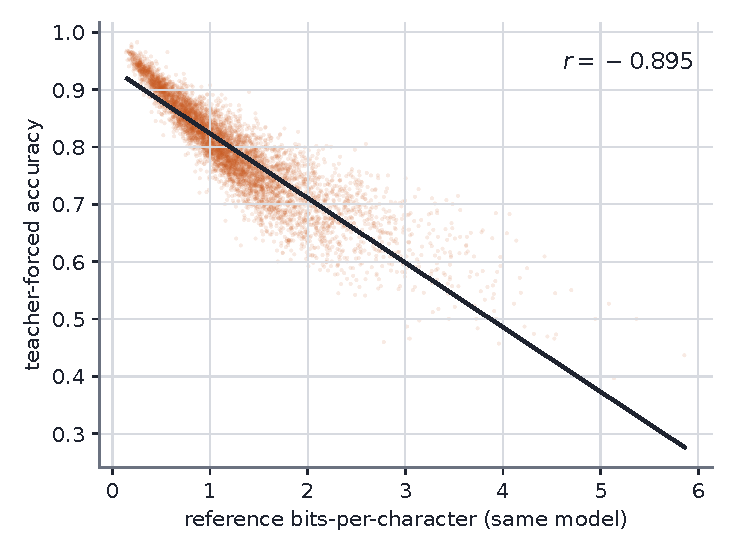
\includegraphics[width=0.55\textwidth]{figures/fig_mechanism.pdf}
\caption{\textbf{Takeaway: to first order, teacher-forced accuracy is reference perplexity. At $r = -0.895$ pooled over 6{,}000 model--item pairs, reference compressibility explains $80\%$ of pooled \tfa{} variance, so the metric meters the reference rather than grading the solution.}
Per-solution \tfa{} against the reference's bits-per-character under the same model on \textsc{MATH-500}, with the least-squares fit.
This pooled view is a corollary of the cross-family decomposition (Table~\ref{tab:decomp}), which is the primary evidence; taken alone it would be partially tautological, since both statistics summarize the same model's prediction fit to the same text.}
\label{fig:mechanism}
\end{figure}

The item effect has a name: reference perplexity.
Across 6{,}000 model--item pairs on \textsc{MATH-500}, \tfa{} correlates with reference perplexity at $r = -0.895$, which explains $80\%$ of the pooled variance (Figure~\ref{fig:mechanism}).
Taken alone this number is partially tautological, since both statistics summarize the same model's prediction fit to the same text, and the model-level fact that likelihood and compression track ability is already established~\cite{huang2024compression,schaeffer2025pretraining,koh2025rbridge}; the correlation is informative here only because the decomposition shows the item effect survives cross-family transfer, which a mere restatement of one model's capability would not need to do.
A score that is four-fifths about the reference cannot grade the solution in front of it.

\paragraph{The result: the interventions.}
Removing the reference's information destroys the ranking signal, and a registered control shows the destruction tracks informativeness rather than token count.
On the same \textsc{MATH-500} items, replacing each worked reference with the single line ``The final answer is [answer]'' collapses the ranking signal from $+0.35$ to $+0.02$ as a point contrast on all seventeen models; the certified statement is the item-level paired bootstrap on the twelve models with per-item data for both variants, a paired delta of $+0.24$ $[+0.12, +0.33]$, excluding zero, while the seventeen-model model-level delta is not distinguishable from zero at that sample size and agrees in sign.
Answer-line references are far shorter than worked ones, so the collapse could partly reflect variance compression from scoring fewer tokens; the registered length-matched control (P-L1) separates the readings, and it landed as predicted.
Each worked reference is replaced by a fixed content-free boilerplate paragraph, identical across items, length-matched to the mean worked reference, and followed by the same answer line: the padded reference keeps per-token predictability high for every model, with a mean \tfa{} of $0.46$ across the same seventeen models, yet it ranks models no better than chance.
On the twelve-model per-item subset the worked references rank at $+0.14$ and the padded references at $-0.27$ over the same 500 items, a paired worked-minus-padded delta of $+0.41$ $[+0.35, +0.46]$, excluding zero decisively; the seventeen-model contrast agrees in sign ($-0.11$ padded versus $+0.35$ worked) but its interval is wide, so we report it as a point contrast only.
Predicting a long, information-dense reference requires skill adjacent to solving the problem; predicting a formulaic one requires nothing, leaving only style.

\subsection{No repair recovers a grade, and one registered call missed}
\label{sec:repairs}

If the variance is reference nuisance, reweighting it cannot mint a grading signal, and the two registered repairs confirm this in opposite directions, one of them against our own registered call.

The position-weighting sweep shows the intuitive repair degrading the metric to negative.
On \textsc{GSM8K}-style data one might weight early reference tokens less than the final ones; with weights $w \propto (\mathrm{pos}/n)^{\gamma}$ over per-token hit vectors for the twelve models with per-token data (this subset's pooled baseline is $+0.13$ rather than $+0.35$), ranking holds near baseline through $\gamma{=}1$, reaches zero by $\gamma \in [4,8]$, and hits $-0.37$ when only the last four tokens count (Figure~\ref{fig:sweeps}, left).
The repair converges to the answer-only-reference null and then overshoots into negative territory, because the variance being redistributed is reference nuisance rather than soundness.
\textbf{The registered prediction was a null; the observed sign flip makes it a miss}, and the register was directionally wrong, not confirmed (Table~\ref{tab:ledger}).

Perplexity normalization is the complementary test, and it empties the metric.
Residualizing reference perplexity out of \tfa{} removes the one thing it robustly measures, and nothing is left: ranking falls from $+0.13$ to $-0.17$, and the item-level signal is null both raw and partialed, as registered.
Seven earlier reweighting variants (IDF, surprisal, masking, and others) predate the registration protocol and all came out $\le 0$.

\section{The boundary: ranking survives exactly where the reference is worth predicting}
\label{sec:p3}

\paragraph{The prediction.}
The reference-predictability nuisance is identical for every model on a given item, so it cancels when scores are averaged over a benchmark; per item it dominates.
Three consequences follow.
Matching should rank models in aggregate while remaining null per solution, a dissociation on the same benchmarks with the same metric; the ranking should hold only where references are informative and models spread, since predicting a dense reference requires skill adjacent to solving the problem; and on saturated benchmarks, where every model predicts the reference about equally well, the leftover variance is family style, so rankings may invert in sign rather than merely fade.
The noisy-grade reading predicts graceful degradation everywhere and forbids the inversion.

\paragraph{The test.}
The boundary map of Table~\ref{tab:map} (page~\pageref{tab:map}): cross-family Spearman between mean \tfa{} and accuracy on nine benchmarks spanning olympiad math to saturated grade-school data, plus twelve hard-side and twelve saturated within-family ladders, and the agentic \textsc{SWE-bench Verified} grid.

\paragraph{The result.}
The boundary lands where the explanation puts it.
The pooled cross-family point estimate runs from $\rho = +0.86$ on olympiad math down through zero to $-0.25$ on \textsc{GSM8K}, the sign inversion the noisy-grade reading forbids; the saturated intervals are wide and straddle zero, so the reversal reading is a point-estimate trend, and the robust statement is the ladder count.
Every family ladder is positive on the three hardest benchmarks with full family coverage, twelve of twelve family--benchmark cells, while on the easiest benchmarks five of twelve ladders invert, Phi on all three saturated benchmarks and OLMo on both \textsc{GSM8K} variants.
Qwen and Mistral stay positive everywhere, a pattern we read as family style canceling inside a family and surviving across families, an interpretive attribution since output style is not directly measured here.
The dissociation is the signature the explanation demands: the same metric that reads $-0.16$ against soundness per solution, and $0.00$ against executed tests per solution, ranks models at $+0.60$ on hard benchmarks, because averaging cancels the item nuisance that drowns the per-solution signal.

The positive side of the boundary is worth stating as plainly as the negative: matching does rank models when three conditions hold at once.
Use it in aggregate, never per item; the reference must be detailed enough to be worth predicting, since neither an answer line nor length-matched boilerplate ranks (Section~\ref{sec:p2}); and the benchmark must be hard enough to differentiate models, since on saturated data the leftover is style.
The agentic setting is consistent with the same boundary, but preliminary: patch-level \tfa{} orders the four Qwen-Coder sizes correctly ($\rho = +1.00$) yet carries no cross-family signal ($\rho = 0.00$, eight models), and a Spearman on a four-model ladder takes only a handful of values.
Across benchmarks the ranking signal correlates $+0.89$ with mean reference perplexity and $-0.81$ with saturation, though the two are confounded observationally, which is exactly why the interventions of Section~\ref{sec:p2} were run.
The consequence for leaderboards: matching is legitimate exactly when these conditions hold, and reference perplexity can be measured in advance, at one forward pass per reference, to check the second one.

\section{What does carry signal, and the registered record}
\label{sec:verify}

\begin{figure}[t!]
\centering
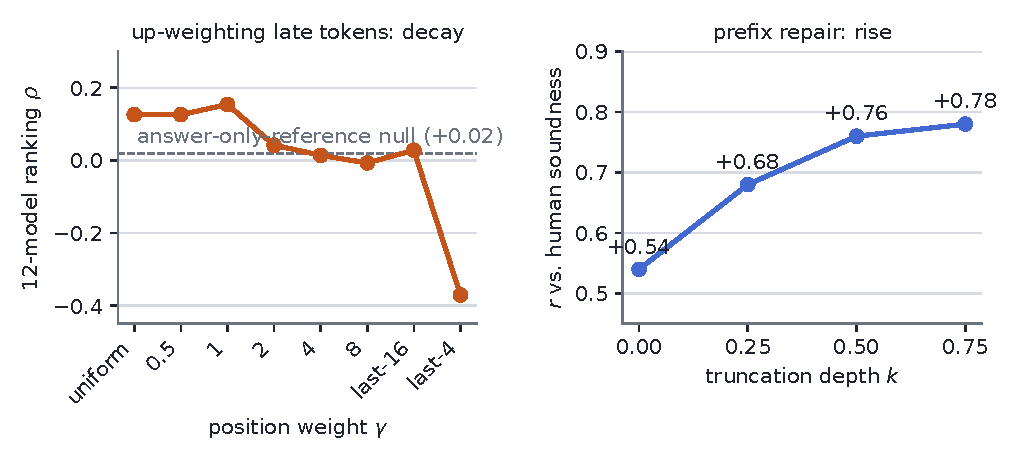
\includegraphics[width=0.88\textwidth]{figures/fig_sweeps.pdf}
\caption{\textbf{Takeaway: repairing a matching metric destroys it while deepening a verification signal strengthens it, but the strengthened signal only converges toward the free bit from below.}
Left: up-weighting late reference tokens decays \tfa's twelve-model ranking signal past $\gamma{=}1$, through the answer-only-reference null and beyond it to $-0.37$ at last-four tokens (the decay is a trend, not strictly monotone: $\gamma{=}1$ ticks up to $+0.15$ and last-16 sits above $\gamma{=}8$); the registered call was a null, so the sign flip is a recorded miss.
Right: the completion-curve signal rises with truncation depth in Pearson, from a pure difficulty probe at $k{=}0$ to $+0.78$ against human soundness at $k{=}0.75$; the dashed line marks the free bit ($+0.92$), which the curve never reaches, and the Spearman profile is non-monotone.}
\label{fig:sweeps}
\end{figure}

An explanation that only forbids is weaker than one that also says where signal lives.
Ours says: any signal that uses the reference solely as a checkable endpoint escapes the nuisance decomposition, because it never scores resemblance to the reference text.
That class prediction was registered and landed for every member tested; what the register did not anticipate is the ordering within the class.

\paragraph{The free bit tops the field.}
Executed tests are the ceiling case, a free correctness oracle wherever they exist and the standard against which \tfa{} scored $0.00$.
On math the analogous baseline is the free answer-correct bit, and it tops everything: on the anchor set it alone correlates $+0.92$ with human soundness.
That correlation is a baseline, not a discovery, since soundness and answer correctness overlap by construction, unsound reasoning usually lands on a wrong answer, and raters may not fully separate the two constructs even under a rubric that asks them to; we therefore treat the bit as the baseline to beat and place the grading question on the within-correct margin.
No signal in this paper beats it.

\paragraph{The completion curve loses to the free bit on paired items.}
The completion curve is the strongest verification signal we built.
Its Pearson correlation with soundness rises with truncation depth, from a pure difficulty probe at $k{=}0$ to $+0.78$ at $k{=}0.75$, and the curve mean reaches $+0.79$ (Figure~\ref{fig:sweeps}, right).
The free bit sits significantly above it: a paired bootstrap of the correlation difference on the same 60 anchor items gives a bit-minus-curve delta of $+0.13$ $[+0.05, +0.24]$, excluding zero.
The partial correlations settle what the curve adds: the curve's partial with soundness given the free bit is $-0.10$, nothing, while the bit's partial given the curve retains $+0.77$.
The honest reading is that the completion curve is a noisy proxy for the free bit wherever the gold final answer is extractable; its residual use case is settings where a final answer cannot be extracted or matched, such as free-form proofs, and that use case is untested here.
Its costs are real, thirty-two completions per solution, and two qualifications travel with the profile: the monotone rise holds in Pearson only, since the Spearman profile is non-monotone, and controlling for difficulty via the $k{=}0$ arm leaves the prefix's added completability at $+0.69$, a partial that does not control for the solution's correctness and so does not rescue a beyond-correctness claim.

\paragraph{A falsified register, and what the falsification teaches.}
We had expected a middle band of completer strength to be required, a completer too weak unable to finish sound work and one too strong rescuing broken work, and registered that expectation as P-C1: washout at 1.5B, gains through 7B, little at 32B.
\textbf{The completed sweep falsifies it}: across Qwen2.5 completers from 1.5B to 32B, a twenty-fold size range over which base solve rates rise sharply, the curve's validity is flat at $+0.78$ to $+0.88$, and the within-correct curve mean stays null at every size.
The washout-at-1.5B leg is decisively falsified, since the 1.5B completer already reaches $+0.78$; the remaining legs are point-wise compatible with the observed ordering but flat within overlapping CIs, so the register as a whole is falsified.
This is a miss for the register and a win for the mechanism, and both statements stand: the middle-band prediction assumed the curve performs graded process evaluation, which should depend on completer strength, and the within-correct nulls say it does not.
On the free-bit reading, any completer strong enough to complete correct reasoning from a sound prefix yields the same correctness signal, and flatness is exactly what that reading predicts.
The curve's magnitude is also not a completer-family artifact: a phi-4 completer on the 42 anchor traces it covers gives a curve mean of $+0.82$ with overlapping intervals, contains zero same-family traces by construction, and reproduces the within-correct null at $+0.02$.

\paragraph{The rest of the class, and the bounds on the nulls.}
The answer-swap check is the cheap end of the class, one forward pass, no judge, no completion: positive in 8 of 9 models with a mean within-model $r$ of $+0.13$, confirming the class prediction in direction while remaining too weak to use alone.
Within the verification class the ordering is led by the cheapest member, the free bit, then the completion curve, then the answer-swap check, and on the within-correct margin none of the cheap signals separates from zero.
The nulls carry equivalence bounds, so the claim is not absence of evidence alone: at $n{=}48$, TOST at $\alpha{=}.05$ excludes within-correct effects larger than about $0.43$ for \tfa, $0.41$ for the curve at $k{=}0.75$, and $0.31$ for the curve mean; effects above roughly $0.4$ are excluded, and moderate effects below that bound cannot be ruled out at this sample size.
The referenced judge's own within-correct value on this random set is $-0.14$, inside a wide interval that straddles zero, so the wide-overlapping-intervals reading holds uniformly, for the judge as well as for the cheap signals, and a cheap beyond-correctness grader remains an open problem.

\begin{table}[tbp]
\centering
\scriptsize
\setlength{\tabcolsep}{2pt}
\resizebox{\textwidth}{!}{%
\begin{tabular}{llllc}
\toprule
register & class & registered prediction & outcome & verdict \\
\midrule
position-weighted \tfa{} & matching & null & ranking decays $+0.13 \to -0.37$ & miss (sign flip) \\
entropy-normalized \tfa{} & matching & null & ranking $+0.13 \to -0.17$; item-level null & hit \\
answer-swap check & verification & carries signal & positive in 8/9 models, mean $+0.13$ & hit \\
completion curve & verification & carries signal & $+0.79$ vs.\ human soundness & hit \\
completer strength (P-C1) & verification & middle band; washout at 1.5B & flat $+0.78$--$+0.88$, 1.5B--32B & falsified \\
length-matched control (P-L1) & matching & ranking stays collapsed & item-level paired delta $+0.41$ $[+0.35,+0.46]$ (worked $-$ padded) & hit \\
\bottomrule
\end{tabular}%
}
\caption{\textbf{Takeaway: four of six registered predictions landed as called, with one sign flip and one falsification on record.}
Each row is one pre-registered directional prediction, committed to the repository before its data were generated.
The class-level divide, verification signals carrying signal where matching carries none, was called in advance, but the register did not anticipate that the free bit would top the class.
The four stronger matching baselines of Section~\ref{sec:p1} were added post hoc in response to review and appear in no row of this ledger.}
\label{tab:ledger}
\end{table}

What the signal-carrying signals share is that none treats the reference text as a target.
Executed tests consume the reference behavior, the free bit and the completion curve use only the reference's final answer as a checkable endpoint, and the answer-swap margin uses that answer as a counterfactual contrast.
Any metric that instead scores resemblance to the reference text inherits the nuisance decomposition of Section~\ref{sec:p2}, which is why the class-level outcome of every entry in Table~\ref{tab:ledger} could be called in advance, even though the free bit's rank within the class could not.
Where LLM judges fall in this taxonomy depends on their protocol; measuring that is the subject of companion work~\cite{companionA}.

\section{Three rules for practice}
\label{sec:rules}

Three rules cover every use of a reference we tested.
\begin{enumerate}
\item \textbf{Check the final answer before buying any deeper signal.}
Wherever the gold final answer is extractable and matchable, the free bit correlates $+0.92$ with blind human soundness on our anchor set, and no signal we tested, matching or verification, adds measurable grading information beyond it.
Reach for completion-based verification only where a final answer cannot be extracted or matched, a setting we have not tested; where you do run it, the completer's strength barely matters, since the curve's validity is flat from a 1.5B to a 32B completer.
\item \textbf{Never use a reference as a similarity target.}
Its value is as context for a reader or as a checkable endpoint for a verifier.
Any metric that scores resemblance to reference text inherits the nuisance decomposition of Section~\ref{sec:p2}, and every repair we or our reviewers proposed failed as the taxonomy expects, one registered call missing in direction (Table~\ref{tab:ledger}); in particular, matching scores should never be used as per-solution rewards or filters.
On math no matching metric clears zero against human soundness, and on code the prediction-fit metrics are indistinguishable from zero against executed tests, with the output-similarity metrics carrying only a weak positive signal far below any grading standard.
\item \textbf{For leaderboards, run a three-step check before trusting matching.}
First, compute mean reference perplexity over the benchmark's references under any strong open model, at one forward pass per reference.
Second, check whether the benchmark is saturated, most models near ceiling, and whether the references are answer lines rather than worked solutions.
Third, if either condition holds, do not use matching; if neither holds, use matching only in aggregate, and report the reference-perplexity figure alongside accuracy so readers can audit the condition.
On answer-line references, matching measures style.
\end{enumerate}

\section{Limitations}
\label{sec:limits}

\paragraph{The human anchor is one small, measured instrument.}
The anchor set is 60 items graded by one annotator who is also an author, with reliability measured rather than assumed: a hypothesis-blind non-author regraded 30 of the 60 under the same rubric on a blinded instrument, agreeing at $0.83$ on soundness, which matches the earlier cross-construct estimate from a shared block.
The replication covers half the anchor items and its intervals are wide, so every ceiling comparison in this paper is indicative only, and the free-baseline partial-correlation nulls inherit the same set's width.
Human-grade validity claims cover one math dataset plus executable code; a second labeled dataset is future work.

\paragraph{The beyond-correctness margin is unresolved.}
Every cheap signal's within-correct value sits inside wide overlapping intervals with no multiplicity correction across the battery, so no cheap signal here demonstrably grades beyond correctness, and the equivalence bounds exclude only effects above roughly $0.4$ at $n{=}48$.
The referenced judge reads $-0.14$ within-correct on the random set, consistent with range restriction without any significance claim, and $+0.81$ only on a divergence-selected stratum of the companion audit~\cite{companionA}, where selection inflates within-correct variance by construction, so its beyond-correctness grading is unresolved as well.

\paragraph{The decomposition is one procedure, and the interventions test one construction.}
The variance shares carry item-level bootstrap intervals and a model-deletion jackknife, but they come from one fixed-effects procedure, so robustness under alternative decomposition procedures remains open; the mechanism claim rests on the decomposition and its cross-family replication, with the interventions as corroboration.
The length-matched control tests one boilerplate template at one length, and other uninformative-reference constructions remain untested.
The item-level paired bootstraps condition on the fixed twelve models, so they capture item-sampling uncertainty only.

\paragraph{Coverage and registration weight are uneven.}
The stronger-baseline block is post hoc and exploratory; two classes remain untested, similarity metrics trained on this task and LLM-based semantic similarity at scale.
The six registered predictions carry first-party git timestamps; the project's pending registered experiments now carry external OSF registrations with third-party timestamps (\texttt{osf.io/jg4ak}, \texttt{osf.io/axp3s}, \texttt{osf.io/ym5x9}, all 2026-08-23), and future registers specific to this paper will follow that practice.
Pooled seventeen-model rankings have wide intervals, so the ranking claims rest on the within-family ladders, which have three to five models each and coarsely quantized Spearmans, read as signs and counts rather than magnitudes; the \textsc{SWE-bench Verified} within-family result rests on a four-model ladder and is a preliminary observation.
All anchor-set numbers come from a single canonical analysis script, and where earlier drafts quoted values from heterogeneous scripts, the canonical values supersede them.

\section{Related work}
\label{sec:related}

\paragraph{Teacher-forced accuracy.}
\tfa{} was introduced by \textsc{Putnam-AXIOM}~\cite{gulati2025putnam} as a judge-free evaluation signal for mathematical reasoning.
This paper does not introduce the metric; it characterizes it, and the result is a corrective map: \tfa{} ranks models where references are worth predicting, saturates and inverts on easy benchmarks, and never grades individual solutions, because most of its per-solution variance belongs to the reference.

\paragraph{Model-level likelihood and ability.}
That model-level likelihood tracks ability is established prior art: compression of held-out text correlates linearly with benchmark performance~\cite{huang2024compression}, and likelihood-based statistics support scaling-law prediction of generative-benchmark scores~\cite{schaeffer2025pretraining} and cross-scale forecasts of reasoning performance~\cite{koh2025rbridge}.
We treat that correlation as known; the delta here is the item-level, cross-family decomposition of the same signal, the saturation boundary it predicts, and the reference interventions that probe the mechanism.

\paragraph{Judges, reference metrics, and biases.}
Reliability audits of LLM judges conclude that reliability without validity is the field's open problem, and call for variance-component analysis of the kind performed here~\cite{zheng2023judging,tan2024judgebench}.
Cheap reference-based metrics descend from text-generation evaluation~\cite{yuan2021bartscore}, where they are typically validated against human preferences of fluency; we test them against blind soundness grades and an executable oracle, and locate their variance in the reference itself.
The style-over-substance literature documents evaluator biases in general response pools~\cite{wu2023style,dubois2024length,singhal2023long}; our contribution is complementary, a mechanism and a corroborating intervention for reference-anchored metrics specifically.

\paragraph{Completion-based verification.}
Completion-based process values descend from rollout estimation in process supervision~\cite{lightman2023verify,wang2022selfconsistency}, and completion-from-prefix scoring is the core of step-level verifiers such as Math-Shepherd~\cite{wang2024mathshepherd} and OmegaPRM~\cite{luo2024omegaprm}.
The completion curve adapts that rollout machinery from reward-model training to judge-free scoring of full solutions against blind human soundness; its depth profile, the class-level advance-prediction test of the matching/verification taxonomy, and the free-baseline comparison showing the curve adds nothing over the free bit on our anchor set are the parts we have not seen in that line.

\section{Conclusion}

Reference-based evaluation has been treated as a spectrum of increasingly good approximations to judgment.
It is not a spectrum; it is two mechanisms, and reading the reference as the owner of the matching score predicts everything we measure while the noisy-grade reading predicts none of it.
No matching metric grades an individual solution, every one landing in $[-0.33, +0.14]$ against blind human soundness with the null replicating against executed tests on code, and the sole escape reads only final answers, the free correctness bit in disguise.
The dominant share of the score's per-solution variance, $83$--$92\%$ for the sharpest metrics, is an item effect that replicates across four model families and has a name, reference perplexity; no reweighting recovers a grading signal, because there is none to recover, and replacing the worked reference with an answer line or with length-matched boilerplate collapses even the ranking signal, the latter under a registered control that landed as called.
And matching ranks models exactly where the reference is worth predicting, positive on every hard-side family ladder, inverting on saturated data where the leftover is style, a boundary a leaderboard can audit in advance by measuring reference perplexity.

The constructive remainder is deflationary in the best sense.
Signals that verify a checkable endpoint carry real signal, but on our anchor set everything they carry is already in the endpoint: the free bit correlates $+0.92$ with human soundness, a baseline expected from construct overlap rather than a discovery, and our strongest verification signal loses to it on paired items and adds nothing given it.
The registered record is four of six predictions landed as called, one sign flip, and one falsification, and the falsification corroborates the mechanism it embarrassed, since a curve that performed graded process evaluation would have depended on completer strength, and it does not.
Check the final answer first, never score resemblance to the reference, and report reference perplexity alongside accuracy; where no final answer can be extracted, a cheap grader that sees beyond correctness remains an open problem, and nothing in the space we tested is it.

\enlargethispage{4\baselineskip}
{\small
\bibliographystyle{plain}
\bibliography{references}
}

\end{document}
